\documentclass[a4paper,amsmath]{oblivoir}

\usepackage{fapapersize}
\usefapapersize{*,*,1in,*,1in,*}

\usepackage{longtable}

\SetHangulspace{1.15}{1}

\makeatletter
\let\ATonum\@onum
\makeatother

\usepackage{efbox}

\usepackage{esgutil}
\usepackage{amsthm}

\usepackage{xcolor}
\usepackage{graphicx}
\usepackage{hologo}
\usepackage{relsize}
\usepackage{tcolorbox}
\tcbuselibrary{listings,breakable}
\tcbset{listing engine=listings,colframe=cyan,colback=cyan!5!white}

\setmainfont{TeX Gyre Pagella}
\setsansfont{Noto Sans}
\setmonofont{Noto Sans Mono}
\setkomainfont(Noto Serif CJK KR)(* Bold)(Noto Sans CJK KR)
\setkosansfont[Noto Sans CJK KR]()( Bold)( Medium)
\usepackage{unicode-math}
\setmathfont{texgyrepagella-math.otf}

\newcounter{sub}
\newcommand\bangotsuite{\stepcounter{sub}\thesub}

\usepackage{tikz}
\newcommand\tikzlogo{Ti\textit{k}Z}
\usetikzlibrary{intersections}

\setlength{\parindent}{0mm}

\newcommand\pkg[1]{\textsf{#1}}

\ExplSyntaxOn 

\NewDocumentEnvironment {intro} {o}
{
    \IfValueTF { #1 }
    {
        \int_set:Nn \l_tmpa_int { #1 }
    }
    {
        \int_set:Nn \l_tmpa_int { 1 }
    }
    \noindent \rule {\linewidth}{3pt}
    \par 
    \sffamily [No.\space\int_use:N \l_tmpa_int ]\ \ 
    \bfseries
}
{
    \hfill \underline{\hphantom{2019}}년~\underline{\hphantom{06}}월~ \underline{\hphantom{25}}일 
    \par 
    \vskip -.3\baselineskip 
    \noindent \rule {\linewidth }{1pt}
    \par 
    \vskip .5\baselineskip 
}

\NewDocumentCommand \exverb { d|| }
{
    \texttt { \tl_to_str:n { #1 } }
}

\ExplSyntaxOff 

\NewDocumentEnvironment {questiona} { m }
{
%    \medskip
    \begin{tcolorbox}[title={#1},fonttitle={\sffamily\bfseries}]
}{%
    \end{tcolorbox}
}

\NewDocumentEnvironment {questionp} { }
{
%    \medskip
    \begin{tcolorbox}[colframe=orange!30!black!60,colbacktitle=orange!25!gray,
    title={연습문제},fonttitle={\sffamily\bfseries}]
}{%
    \end{tcolorbox}
}


\NewDocumentEnvironment {exampleonly} {}
{%
%    \begin{tcblisting}{listing only}
    \expandafter\tcblisting{listing only,breakable,before={\par\medskip\setstretch{1}}}
}{
    \endtcblisting
%    \end{tcblisting}
}

\NewDocumentEnvironment {exampleside} {}
{%
    \tcblisting{listing side text,breakable,before={\par\medskip\setstretch{1}}}%
}{%
    \endtcblisting
}

%\NewDocumentEnvironment {examplebelow} {}
%{%
%    \medskip
%    \tcblisting{text below listing,breakable}%
%}{%
%    \endtcblisting
%}
\newtcblisting{examplebelow}{breakable,before={\par\medskip\setstretch{1}},listing options={numbers=left,stepnumber=1,basicstyle=\small\ttfamily,breaklines=true}}

\begin{document}

\title{정답과 해설}
\author{esg004}
\date{2019/07/15}

\maketitle

\begin{questionp}

\fbox{기본} 1. 본문의 예제는 루프를 탈출하기 위하여 \verb|\clist_map|을 활용하였다.
그런데 while do를 쓰면 clist mapping을 이용하지 않아도 루프의 탈출 조건을 
만들 수 있다. 이를 이용하여 같은 알고리즘을 구현할 수 있겠는가?
\end{questionp}

이 문제의 출제 취지는 “while do”의 탈출 조건을 구성하는 것을 보겠다는 것이었습니다.
충분히 이해하고 있는 것으로 보입니다. 이 문제를 해결하는 알고리즘을 다시 정리하면 다음과 같습니다.
\begin{enumerate}[\expandafter\ATonum1] \firmlist
\item 주어진 수를 $N$이라 하면, 2부터 N (또는 N-1)까지 다음 과정을 반복
\item 반복할 때의 수를 $n$이라 하고, 이것을 나누어볼 수를 $p$.
\item “소수이다”를 나타내는 boolean을 true로 설정
\item $p$를 2부터 1 증가시켜가면서 $n$\%$p$==0인지를 검사하여 나누어지면 bool을 false로.
\item 나누어질 수 $n$의 제곱근보다 $p$가 커지거나 (다르게 하면 $p^2$가 $n$보다 커지는지를 검사) 또는 bool이 false이면 탈출
\item bool이 true이면 소수이므로 clist에 $n$을 추가
\end{enumerate}

이것을 expl3로 쓰면 다음과 같이 할 수 있습니다.

\begin{examplebelow}
\ExplSyntaxOn
\int_new:N \l_n_int
\int_new:N \l_p_int

\clist_new:N \l_primes_clist
\bool_new:N \l_prime_bool

\cs_new:Npn \primes_le_num:n #1
{
    \clist_clear:N \l_primes_clist
    
    \int_set:Nn \l_n_int { 2 }
    
    \int_while_do:nn { \l_n_int <= #1 }
    {
        \int_set:Nn \l_p_int { 2 }
        \bool_set_true:N \l_prime_bool
        
        \bool_while_do:nn
        {
            \int_compare_p:n { \l_p_int * \l_p_int <= \l_n_int }
            &&
            \l_prime_bool
        }
        {
            \int_compare:nT { \int_mod:nn { \l_n_int } { \l_p_int } == 0 }
            {
                \bool_set_false:N \l_prime_bool
            }
            \int_incr:N \l_p_int
        }
        
        \bool_if:NT \l_prime_bool
        {
            \clist_put_right:No \l_primes_clist { \int_use:N \l_n_int } 
        }
        
        \int_incr:N \l_n_int
    }
}

\primes_le_num:n { 100 }
\clist_use:Nn \l_primes_clist {,~}

\ExplSyntaxOff

\end{examplebelow}

두 가지 탈출조건을 충족하기 위해서 \verb|\bool_while_do:|와 boolean 연산을 썼습니다.

\paragraph{숙제에 대한 코멘트}
이재호 군은 탈출조건을 만들 필요가 없는 바깥쪽 루프를 \verb|\int_step_...|으로 처리하고
안쪽은 \verb|\bool_while_do:Nn \l_tmpa_bool|을 이용하였는데,
n이 p로 나누어떨어지지 않으면 true, 그리고 floor(sqrt(n))보다 작거나 같으면 true로
하고 이 변수의 boolean 값을 검사하여 반복시키는 방법을 썼습니다. 근본 발상은 위에 소개한 
것과 동일하고 잘 해결하였습니다.

\medskip

신현 군은 boolean을 전혀 쓰지 않고 정수 계산만으로 다음과 같은 코드를 보여주었습니다.
복잡한 “두 가지 조건”에 구애받지 않고 “나누어지는가”만 문제삼은 코드인데, 문제에 대한 해결이 되었다고
봅니다.
\begin{exampleonly}
\cs_new:Npn \get_factors:n #1
{
    \int_set:Nn \l_N_int { #1 }
    \int_set:Nn \l_p_int { 2 }
    
    \int_while_do:nn { \l_N_int >= \l_p_int }
    {
        \int_set:Nn \l_i_int { 2 }
        \int_set:Nn \l_chk_int { 1 }
        \int_while_do:nn { \l_p_int > \l_i_int }
        {
            \int_compare:nT { \int_mod:nn { \l_p_int } { \l_i_int } == 0 }
            {
                \l_chk_int = 0
            }
            \int_incr:N \l_i_int
        }
        
        \int_compare:nT { \l_chk_int == 1 }
        {
            \clist_gput_right:No \g_factors_clist { \int_use:N \l_p_int }
        }
        \int_incr:N \l_p_int
    }
}
​\end{exampleonly}


\newpage

\begin{questionp}
\fbox{발전} 2. 주어진 수가 소수인지를 검사하는 다음과 같은 알고리즘이 있다. 이를 expl3로 구현할 수 있겠는가?

\medskip

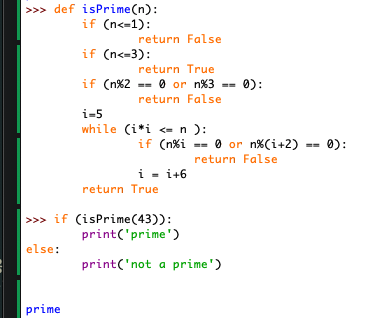
\includegraphics[scale=.78]{Screenshot-2}
\end{questionp}

\begin{examplebelow}
\ExplSyntaxOn
\bool_new:N \g_isprime_bool

\cs_new:Npn \is_prime:n #1
{
    \int_case:nnF { #1 }
    {
        { 0 } { \bool_gset_false:N \g_isprime_bool }
        { 1 } { \bool_gset_false:N \g_isprime_bool }
        { 2 } { \bool_gset_true:N  \g_isprime_bool }
        { 3 } { \bool_gset_true:N  \g_isprime_bool }
    }
    {
        \bool_if:nTF
        {
            \int_compare_p:n { \int_mod:nn { #1 } { 2 } == 0 }
            ||
            \int_compare_p:n { \int_mod:nn { #1 } { 3 } == 0 }
        }
        {
            \bool_gset_false:N \g_isprime_bool
        }
        {
            \do_check_prime:n { #1 }
        }
    }
    
    \bool_if:NTF \g_isprime_bool
    {
        #1~is~prime. \par
    }
    {
        #1~is~composite.\par
    }
}

\int_new:N \l_i_int

\cs_new:Npn \do_check_prime:n #1
{
    \int_set:Nn \l_i_int { 5 }
    \bool_set_true:N \g_isprime_bool
    
    \bool_do_while:nn 
    {
        \int_compare_p:n { \l_i_int * \l_i_int <= #1 }
        &&
        \g_isprime_bool
    }
    {
        \bool_if:nT 
          {
            \int_compare_p:n { \int_mod:nn { #1 } { \l_i_int } == 0 }
            ||
            \int_compare_p:n { \int_mod:nn { #1 } { \l_i_int + 2 } == 0 }
          }
          {
            \bool_gset_false:N \g_isprime_bool
          }

        \int_add:Nn \l_i_int { 6 }
    }
}

\is_prime:n { 227 }

\is_prime:n { 2019 }
\ExplSyntaxOff
\end{examplebelow}

이 코드를 “번역”할 때 주의하여야 할 것은 python의 return문입니다. return은 그 위치에서 함숫값을 반환하고 “종료”합니다. 그러나 expl3에는 return이란 게 없다는 사실을 기억합니다.

그렇기 때문에 \verb|\bool_while_do|하면서 “나누어보는 수”의 제곱이 주어진 수보다 (누누이 설명한 바 제곱근을 넘지 않는 최대 정수) 크지 않고 “소수가 아님이 판명되지 않은” 조건에서 반복하도록 했습니다(line 44--49).
이는 while 문의 탈출 조건을 만든 것입니다.

\paragraph{숙제에 대한 코멘트}
이재호 군의 풀이는 위에 예시한 코드와 거의 동일하여, 정답이라고 할 만합니다.

신현 군의 풀이는 1번과 마찬가지로 \verb|\l_chk_int| 값을 0로 만들면 false가 되도록 문제를 해결하려 하였습니다. 한 가지 해결방법이 되겠지요, 다음은 신현 군이 보내온 코드를 완성해본 것입니다.

\begin{exampleonly}
\int_new:N \l_chk_int
​
\NewDocumentCommand \primes { m }
{
    \thisisfunction:n { #1 }
    \int_compare:nTF { \l_chk_int == 0 }
    {
        Not~a~Prime
    }
    {
        Prime
    }
}
​​
\int_new:N \l_N_int
\int_new:N \l_p_int
\int_new:N \l_i_int
\int_new:N \l_n_int
​
​\cs_new:Npn \thisisfunction:n #1
{
    \int_set:Nn \l_N_int { #1 }
    \int_set:Nn \l_chk_int { 1 }
    \int_set:Nn \l_i_int { 5 }
    
    \int_compare:nT { \l_N_int <= 1 }
    {
        \l_chk_int = 0
    }
​
    \int_compare:nT { ((\l_N_int+1)/2) == 2 }
    {
        \l_chk_int = 2
    }
​
    \int_compare:nT { \l_chk_int == 1 }
    {
        \int_compare:nT { \int_mod:nn { \l_N_int } {2} == 0 }
        {
            \l_chk_int = 0
        }
        \int_compare:nT { \int_mod:nn { \l_N_int } {3} == 0 }
        {
            \l_chk_int = 0
        }
    }
​
    \int_set:Nn \l_i_int { 5 }
    
    \int_compare:nT { \l_chk_int == 1 }
    {
        \int_while_do:nn { \l_N_int >= \l_i_int * \l_i_int }
        {
            \int_compare:nT { \int_mod:nn { \l_N_int } { \l_i_int } == 0 }
            {
                \l_chk_int = 0
            }

            \int_compare:nT { \int_mod:nn { \l_N_int } { \l_i_int+2 } == 0 }
            {
                \l_chk_int = 0
            }

            \int_add:Nn \l_i_int { 6 }
        }
    }
​}
\end{exampleonly}

\newpage

\begin{questionp}
\fbox{실력} 3. KTUG 게시판 \href{http://www.ktug.org/xe/index.php?document_srl=235888&mid=KTUG_open_board}{:235888} 글에 소인수분해 알고리즘이 소개되어 있다. 
이를 바탕으로 다음 순서로 문제를 해결하여라.
\begin{enumerate}[\ \ \expandafter\ATonum1] \firmlist
\item 두 수를 인자로 받아서 최대공약수를 구하여라.
\item 최대공약수를 소인수분해하여 결과를 clist나 seq에 저장하여라.
\item 최대공약수의 소인수를 취하여 차례로 두 수를 나누어가면서 몫(quotient)의 변화 과정을 clist나 seq에 저장하여라.
\item 준비된 세 개의 clist (seq)를 이용하여 다음 그림과 같이 출력하여라.
\end{enumerate}
\begin{center}
\begin{tabular}{r|rr}
2 & 16 & 24 \\ \cline{2-3}
2 & 8  & 12 \\ \cline{2-3}
2 & 4 & 6 \\ \cline{2-3}
  & 2 & 3 \\ 
\end{tabular}
\end{center}
\end{questionp}

\textbf{\ATonum 1 최대공약수 구하기}

최대공약수는 이미 구해보았습니다. 여기서는 구한 최대공약수를 “출력”하는 것이 아니라 
전역변수 하나에 보관하도록 처리합니다. 

\begin{examplebelow}
\ExplSyntaxOn

\int_new:N \g_gcd_int
\int_new:N \l_a_int
\int_new:N \l_b_int
\int_new:N \l_c_int

\cs_new:Npn \gen_gcd:nn #1 #2 
{
    \int_set:Nn \l_a_int { \int_max:nn { #1 } { #2 } }
    \int_set:Nn \l_b_int { \int_min:nn { #1 } { #2 } }
    
    \int_while_do:nn { \l_b_int != 0 }
    {
        \int_set:Nn \l_c_int { \int_mod:nn { \l_a_int } { \l_b_int } }
        \int_set_eq:NN \l_a_int \l_b_int
        \int_set_eq:NN \l_b_int \l_c_int
    }
    
    \int_gset_eq:NN \g_gcd_int \l_a_int
}

%%%%%%%%%% ==== test ====
\gen_gcd:nn { 14 } { 49 }  \int_use:N \g_gcd_int
\ExplSyntaxOff
\end{examplebelow}

\bigskip

\textbf{\ATonum 2 최대공약수의 소인수분해}

링크된 글에 나오는 소인수분해 알고리즘은 다음과 같습니다. 어려운 점은 없다고 봅니다.

\begin{tcblisting}{listing only,listing options={language=Python}}
N = int( input("Enter a number : ") )
p = 2
F = []
while N >= p**2:
    if N%p == 0:
        F.append(p)
        N = N/p
    else:
        p = p+1
F.append(int(N))
\end{tcblisting}

이를 expl3로 구현하면서, 얻어지는 소인수들을 \verb|\g_factors_clist|에 저장하겠습니다.
원한다면 seq로 해도 상관없습니다.

\begin{examplebelow}
\ExplSyntaxOn
\clist_new:N \g_factors_clist
\int_new:N \l_N_int
%\int_new:N \l_p_int

\cs_new:Npn \gen_factors:n #1
{
    \clist_clear:N \g_factors_clist
    \int_set:Nn \l_p_int { 2 }
    \int_set:Nn \l_N_int { #1 }
    
    \int_while_do:nn { \l_N_int >= \l_p_int * \l_p_int }
    {
        \int_compare:nTF { \int_mod:nn { \l_N_int } { \l_p_int } == 0 }
        {
            \clist_gput_right:Nx \g_factors_clist { \int_use:N \l_p_int }
            \int_set:Nn \l_N_int { \l_N_int / \l_p_int }
        }
        {
            \int_incr:N \l_p_int
        }
    }
    
    \clist_gput_right:Nx \g_factors_clist { \int_use:N \l_N_int }
}

%%%%%% ==== test ====
\gen_factors:n { 72 }
\clist_use:Nn \g_factors_clist { , ~ }

\ExplSyntaxOff
\end{examplebelow}

\verb|\g_gcd_int|와 \verb|\g_factors_clist|는 이후 다른 함수에서 참조하는 
변수들이므로 이런 경우에는 스크래치 변수를 사용하지 않는 편이 좋습니다.
예전 “원시 \TeX” 시절에는 레지스터 개수의 제한 때문에 새로운 변수 할당에 많은 
고민이 필요했습니다만 지금 \TeX 은 웬만해서 레지스터가 부족한 문제는 잘 발생하지 않습니다.

\bigskip

\textbf{\ATonum 3 몫의 변화 추적}

일단, clist로 주어지는 소인수들로 어떤 수를 차례로 나누어 가면서 몫을 clist에 저장해야 하므로,
“어떤 수”, “소인수 clist”, “결과를 저장할 clist” 세 개의 인자를 받는 명령을 작성합니다.
그러면 인자형은 \verb|:nNN| 형이 될 것입니다.

그런데 이 함수는 성격상 재귀적으로 정의하는 것이 좋을 듯해요. 재귀 호출이 이루어지는 시점에서 
첫 번째 인수는 아마도 매크로 정수일 테니까 이것을 호출하기 위해서 \verb|:VNN| 꼴의 variant를
만들어둡시다.

재귀 호출의 중단조건은 “소인수 clist”가 모두 소진되는 때입니다. 

소인수 clist에서 하나씩 꺼내어 나누기를 시행하는 때, \verb|\clist_item:Nn|을 이용해도 좋고,
소인수 clist의 임시 복사본을 만들어두고 \verb|\clist_pop:NN|으로 간단히 꺼내는 것도 좋은 
방법입니다. 대체로 말해서 \verb|\clist_pop:NN|이 훨씬 안전한데 그 이유는 \verb|\clist_item:Nn|의
결과를 특정 변수에 넣고 사용하려 할 때 “확장” 관련 문제가 발생할 확률이 \verb|\clist_pop|보다
높기 때문입니다. 그러니까 혹시 \verb|\clist_item:Nn|이 뜻대로 동작하지 않으면 popping을 시도해보기
바랍니다.

\begin{examplebelow}
\ExplSyntaxOn
\cs_new:Npn \trace_quot:nNN #1 #2 #3
{
    \clist_set:Nn #3 { #1 }
    
    \int_zero:N \l_tmpa_int
    
    \trace_quot_rec:nNN { #1 } #2 #3
}

\cs_new:Npn \trace_quot_rec:nNN #1 #2 #3
{
    \int_incr:N \l_tmpa_int
    
    \int_compare:nT { \l_tmpa_int <= \clist_count:N #2 }
    {
        \tl_set:Nx \l_tmpa_tl { \clist_item:Nn #2 { \l_tmpa_int } } 
        \int_set:Nn \l_tmpb_int { #1 / \l_tmpa_tl }
        \clist_put_right:Nx #3 { \int_eval:n { \l_tmpb_int } }
        \trace_quot_rec:VNN \l_tmpb_int #2 #3
    }
}

\cs_generate_variant:Nn \trace_quot_rec:nNN { VNN }

%%%% ==== test ====
\clist_set:Nn \l_tmpa_clist { 2, 2, 2, 3 }
\trace_quot:nNN { 24 } \l_tmpa_clist \l_tmpb_clist
\clist_use:Nn \l_tmpb_clist {,~ }
\ExplSyntaxOff
\end{examplebelow}

line 4: \\
결과 저장 clist를 비우지 않고 맨 첫 항목으로 인자로 들어온 수를 넣었습니다.
위의 test 코드를 보면 바로 알 수 있을 겁니다.

\medskip

line 6: \\
인덱스 카운터를 초기화하는 것을 재귀적으로 호출되는 함수 내에서 하면 안 됩니다.
재귀 함수를 별도로 정의한 것은 이 때문입니다.

\medskip

재귀적으로 정의하지 않아도 문제를 해결할 수 있을 거여요. 어차피 clist는 유한한 항목을
가지고 있고 각 항목 순서가 정해져 있으니까요. 흥미가 있다면 이것을 시도해보아도 좋습니다.

\bigskip

\textbf{\ATonum 4 명령 작성}

우리가 만들고자 하는 명령은 \verb|\drawfactor|. 두 개의 정수를 받아서
(1) 먼저 최대공약수를 구하고,
(2) 그 최대공약수를 소인수분해하고
(3) 두 수를 각각 소인수들로 나누어서 몫을 저장하는 것까지 진행해보겠습니다.

\begin{examplebelow}
\ExplSyntaxOn

\cs_generate_variant:Nn \gen_factors:n { V }

\clist_new:N \l_qa_clist
\clist_new:N \l_qb_clist

\NewDocumentCommand \drawfactor { m m }
{
    \gen_gcd:nn { #1 } { #2 }
    \gen_factors:V \g_gcd_int
    \trace_quot:nNN { #1 } \g_factors_clist \l_qa_clist
    \trace_quot:nNN { #2 } \g_factors_clist \l_qb_clist
}

%%%% === test ===
\drawfactor{16}{24}
f:~ \clist_use:Nn \g_factors_clist {,~} \\
a:~ \clist_use:Nn \l_qa_clist {,~} \\
b:~ \clist_use:Nn \l_qb_clist {,~}
\ExplSyntaxOff
\end{examplebelow}

일단 모든 clist들이 원하는 모양을 갖추었음을 알 수 있습니다.
이제 이것으로 그림을 그려야 하는데, tabular로 그리는 경우

\ExplSyntaxOn
\NewDocumentCommand \drawfactor { m m }
{
    \gen_gcd:nn { #1 } { #2 }
    \gen_factors:V \g_gcd_int
    \trace_quot:nNN { #1 } \g_factors_clist \l_qa_clist
    \trace_quot:nNN { #2 } \g_factors_clist \l_qb_clist
}
\ExplSyntaxOff

\begin{examplebelow}
\ExplSyntaxOn
\drawfactor{16}{24}
\begin{tabular}{r|rr}
\int_step_inline:nn { \clist_count:N \g_factors_clist }
{
    \clist_gpop:NN \g_factors_clist \l_tmpa_tl \tl_use:N \l_tmpa_tl &
    \clist_gpop:NN \l_qa_clist \l_tmpa_tl \tl_use:N \l_tmpa_tl &
    \clist_gpop:NN \l_qb_clist \l_tmpa_tl \tl_use:N \l_tmpa_tl \\ \cline{2-3}
}
    &
    \clist_gpop:NN \l_qa_clist \l_tmpa_tl \tl_use:N \l_tmpa_tl &
    \clist_gpop:NN \l_qb_clist \l_tmpa_tl \tl_use:N \l_tmpa_tl \\ 
\end{tabular}
\ExplSyntaxOff
\end{examplebelow}

이렇게 되네요. 이것으로 좋지만 여기서는 \textsf{efbox}라는 것을 
이용하는 방법도 써보기로 하고 예시 코드만 보이겠습니다. \textsf{efbox} 패키지와
명령 \verb|\efbox|의 사용법은 패키지 문서를 읽어보세요.

\begin{examplebelow}
\ExplSyntaxOn
\RenewDocumentCommand \drawfactor { m m }
{
    \gen_gcd:nn { #1 } { #2 }
    \gen_factors:V \g_gcd_int
    \trace_quot:nNN { #1 } \g_factors_clist \l_qa_clist
    \trace_quot:nNN { #2 } \g_factors_clist \l_qb_clist
    
    \draw_tabular_from_clists:NNN \g_factors_clist \l_qa_clist \l_qb_clist
}

\def\clinenewline { \tabularnewline }

\cs_new:Npn \draw_tabular_from_clists:NNN #1 #2 #3
{
    \tl_clear:N \l_tmpa_tl
    \begin{minipage}[t]{8em}
        \int_step_inline:nn { \clist_count:N #1 }
        {
            \tl_put_right:Nn \l_tmpa_tl 
            {
                \efbox [hidealllines] { \makebox [ 1em ] [r] { \clist_item:Nn #1 { ##1 } } \hspace{1em} }
                \efbox [topline=false, rightline=false] { \makebox [ 2em ] [r] { \clist_item:Nn #2 { ##1 } } }
                \efbox [topline=false, rightline=false, leftline=false] { \makebox [ 2em ] [r] { \clist_item:Nn #3 { ##1 } } }
                \newline
            }
        }
        
        \l_tmpa_tl
    
        \efbox [hidealllines] { \makebox [ 1em ] [r] {  } \hspace{1em} }
        \tl_set:Nn \l_tmpb_tl { \clist_item:Nn #2 { \clist_count:N #2 } }
        \efbox [linecolor=white,topline=false, rightline=false] { \makebox [ 2em ] [r] { \l_tmpb_tl } }
        \tl_set:Nn \l_tmpb_tl { \clist_item:Nn #3 { \clist_count:N #3 } }
        \efbox [linecolor=white,topline=false, rightline=false, leftline=false] { \makebox [ 2em ] [r] { \l_tmpb_tl } }
    \end{minipage}
}
\ExplSyntaxOff

\drawfactor{16}{24} 
\drawfactor{108}{9}
\end{examplebelow}

\paragraph{숙제에 대한 코멘트}
이 문제는 아마 처음으로 제대로 된 \LaTeX{} 명령 하나를 작성해보는 연습이 되었을 거여요.
해결책은 구상이 되었고 구현도 가능할 듯하지만 상당한 시간을 요하는 문제라서
아마 시간 부족으로 끝을 내지 못한 것으로 이해합니다.

\newpage

\begin{questionp}

\fbox{기본} 1. 가로 10cm, 세로 10cm이고 상하좌우 여백이 1.5cm, 모두 30페이지를 가진 pdf 문서를 작성한다. 매 페이지마다 현재 페이지가 전체 페이지수에 대하여 몇 \%인지를 표시하고 페이지 번호가 5의 배수가 되는 때 페이지의 배면색상(background color)를 cyan으로 하여라.
\end{questionp}

한 페이지만 색상을 달리 하려 할 때,
\begin{verbatim}
\usepackage{pagecolor,afterpage}
\end{verbatim}
이것을 preamble에서 선언하고

\begin{verbatim}
\pagecolor{<color>}
\afterpage{\nopagecolor}
\end{verbatim}

이것은 고전적이고 표준적 방법입니다. 꼭 기억해두세요.

pdf의 사이즈를 정하는 문제는 \textsf{memoir}를 읽었으므로
\begin{verbatim}
\settrimmedsize{10cm}{10cm}{*}
\setulmargins{1.5cm}{*}{*}
\setlrmargins{1.5cm}{*}{*}
\checkandfixthelayout
\end{verbatim}
이와 같이 할 수 있겠으나 \textsf{fapapersize}라는 너무나 좋은 \verb|:-)| 패키지가
있으므로 이것을 이용하지요.

\begin{exampleonly}
\documentclass{oblivoir}

\usepackage{fapapersize}
\usefapapersize{10cm,10cm,1.5cm,*,1.5cm,*}
\usepackage{xcolor,pagecolor,afterpage}

\begin{document}

\ExplSyntaxOn

\int_compare:nTF { \thelastsheet == 0 }
{
    \fp_set:Nn \l_tmpa_fp { 1 }
}
{
    \fp_set:Nn \l_tmpa_fp { \thelastsheet }
}

\int_step_inline:nn { 30 }
{
    \begin{vplace}
    \centering
    \fp_eval:n { \thepage / \l_tmpa_fp * 100 } \%
    \end{vplace}
    
    \int_compare:nT { \int_mod:nn { \thepage } { 5 } == 0 }
    {
        \pagecolor{cyan!80}
        \afterpage{\nopagecolor}
    }

    \newpage
}

\ExplSyntaxOff

\end{document}
\end{exampleonly}

\textsf{memoir}가 제공하는 \verb|\thelastpage|와 \verb|\thelastsheet|는 
매우 중요한 매크로입니다. 직관적으로 알 수 있겠지만 매뉴얼의 해당 부분을 읽어두세요.

\verb|\thelastsheet|는 처음에 0으로 되어 있습니다. 이걸 그냥 두면 0으로 나누기 에러가 발생할
위험이 있으므로 이 값이 정해지기까지(즉 한 번 컴파일할 때까지) 에러 처리 코드를 두었습니다.
두 번째 컴파일에서 원하는 결과가 나올 것입니다.

\newpage

\begin{questionp}
\fbox{기본} 2. 위의 pdf 문서 각 페이지의 중앙에 반지름 3cm인 원을 그리고 진행비율(현재페이지/전체페이지)을 붉은 색으로 표시하는 progress pie를 그려라.
\end{questionp}

색상 있는 arc를 그리는 문제는 \tikzlogo{} 관련 문제이므로 별도로 설명하지 않습니다.

\begin{exampleonly}
\documentclass{oblivoir}

\usepackage{fapapersize}
\usefapapersize{10cm,10cm,1.5cm,*,1.5cm,*}
\usepackage{xcolor,pagecolor,afterpage}
\usepackage{tikz}

\begin{document}

\ExplSyntaxOn

\int_compare:nTF { \thelastsheet = 0 }
{
    \int_set:Nn \l_tmpa_int { 1 }
}
{
    \int_set:Nn \l_tmpa_int { \thelastsheet }
}

\int_step_inline:nn { 30 }
{
%%% draw pie
    \fp_set:Nn \l_tmpa_fp { \thepage / \l_tmpa_int * 100 } 
    \fp_set:Nn \l_tmpb_fp { \l_tmpa_fp * 360 / 100 - 90 }
    \tl_set:Nx \l_tmpa_tl { \fp_use:N \l_tmpb_fp }
    \begin{tikzpicture}[remember~picture,overlay]
      \draw (current~page.center) circle (3cm);
      \filldraw [red,fill=red] (current~page.center) -- +(0,3) arc (90\c_colon_str -\l_tmpa_tl \c_colon_str 3) -- cycle;
      \node at (current~page.center) { \fp_eval:n { round ( \l_tmpa_fp, 2 ) } \% };
    \end{tikzpicture}

%%% coloring page
    \int_compare:nT { \int_mod:nn { \thepage } { 5 } == 0 }
    {
        \pagecolor{cyan!50}
        \afterpage{\nopagecolor}
    }

    \newpage
}

\ExplSyntaxOff

\end{document}
\end{exampleonly}

\newpage

\begin{questionp}
\fbox{기본} 3. 중학교 수학 교과서의 부록으로 “삼각비표”가 있다. 이 표의 일부 ($0^\circ$부터 $25^\circ$까지)를 되도록 예쁘게 작성하여라.
\end{questionp}

삼각\dotemph{비}표이므로 $0^\circ$에서 정의되지 않습니다(삼각함수표라면 얘기가 다르겠지만).
degree 삼각함수를 써야 한다는 점 말고는 주의할 것이 없어요. 

이 표는 기본적으로 한 페이지에 다 그리지 못할 가능성이 있으므로 \textsf{longtable}을 사용하는 것이 좋습니다.

“예쁘게” 부분을 무시하고 결과를 보이면,

\begin{examplebelow}
\ExplSyntaxOn

\begin{longtable}{r|rrr}
\hline
deg & $\sin$ & $\cos$ & $\tan$ \\ \hline
\endhead
0 & N/A & N/A & N/A \\ \hline
\int_step_inline:nn { 24 }
{
    #1 & 
    \fp_eval:n { round ( sind ( #1 ), 4 ) } & 
    \fp_eval:n { round ( cosd ( #1 ), 4 ) } & 
    \fp_eval:n { round ( tand ( #1 ), 4 ) } 
    \\ \hline
}
25 & 
\fp_eval:n { round ( sind ( 25 ), 4 ) } & 
\fp_eval:n { round ( cosd ( 25 ), 4 ) } & 
\fp_eval:n { round ( tand ( 25 ), 4 ) } \\ \hline
\end{longtable}

\ExplSyntaxOff
\end{examplebelow}

더 보기좋게 하려면 지난 주에 배운 \verb|\format_num:n|을 적용할 수 있습니다.

\paragraph{숙제에 대한 코멘트}

박승원 군이 이 문제를 다음과 같이 해결했는데요,
\begin{exampleonly}
\ExplSyntaxOn
\begin{center}
\begin{tabular}{|c|c|}
\hline
$ x $ & $ \sin{x} $ \\
\hline
\int_step_inline:nnn { 0 } { 25 }
{%
    #1 & \fp_eval:n { round( sin ( #1 * pi / 180 ) , 4 ) } \\
}%
\hline
\end{tabular}
\end{center}
\ExplSyntaxOff
\end{exampleonly}
\verb|sind| 함수 대신 deg를 rad로 바꾸고 그 값에 \verb|sin|을 취했네요.

그리고 위의 코드는 tabular 관련 대표적 에러 중의 하나인 \verb|\noalign| 에러를 만날 것입니다.
그 이유는 \verb|\int_step_...|이 마지막에 loop를 중단하는 quark들이 몇 개 들어가는데
이것이 확장되면서 새로운 tabular line이 시작한 것처럼 tabular가 인식하기 때문이에요.
그러니까 24행까지만 step함수를 쓰고 마지막 행은 직접 적어줍니다. 
\begin{examplebelow}
\ExplSyntaxOn
\begin{center}
\begin{tabular}{|c|c|}
\hline
$ x $ & $ \sin{x} $ \\
\hline
\int_step_inline:nnn { 0 } { 4 }
{
    #1 & \fp_eval:n { round( sin ( #1 * pi / 180 ) , 4 ) } \\
}
    5 & \fp_eval:n { round( sin ( 5 * pi / 180 ) , 4 ) } \\
\hline
\end{tabular}
\end{center}
\ExplSyntaxOff
\end{examplebelow}




\newpage

\begin{questionp}
\fbox{실력} 4. 다음 그림을 그려보아라. 배경색은 별도로 지정하지 않아도 좋다.

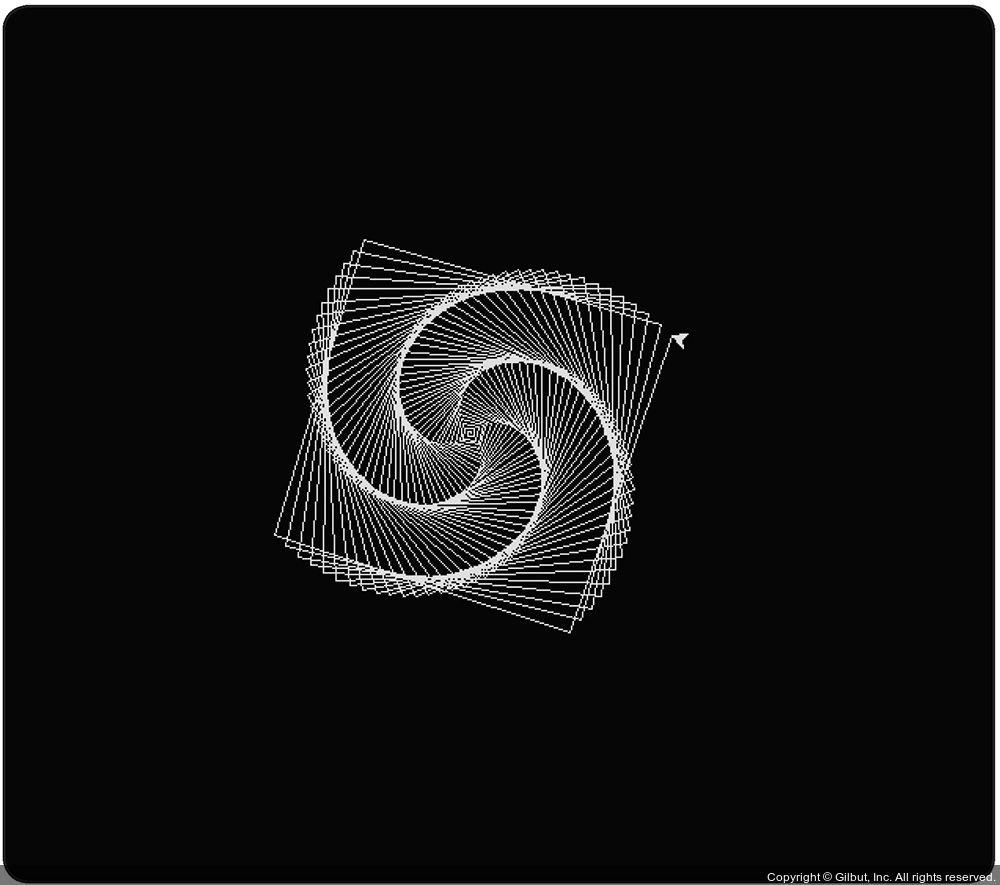
\includegraphics[width=.7\linewidth]{Screenshot-4}

\end{questionp}

python turtle 모듈로 이 그림을 그리는 코드가 다음과 같습니다.

\begin{tcblisting}{listing only,listing options={language=Python}}
import turtle as t
angle=89
for x in range(200):
    t.forward(x)
    t.left(angle)
\end{tcblisting}

조인성 교수께서 제공하신 해법(마지막에 전체 소스를 붙였습니다)으로 이 코드를
구현하면 다음과 같이 됩니다.

\begin{examplebelow}
\ExplSyntaxOn
\tl_set:Nn \l_angle_tl { 89 }
\tl_set:Nn \l_multiplier_tl { 0.02 }

\cs_new:Npn \build_turn_box:n #1
{
    \tl_clear:N \l_tmpa_tl
    \int_step_inline:nn { #1 }
    {
        \tl_put_right:Nx \l_tmpa_tl
        {
            -- ( [turn] 89\c_colon_str \fp_eval:n { \l_multiplier_tl * ##1 } )
        }
    }
    
    \tl_put_left:Nn \l_tmpa_tl { (0,0) }
}

%%%% === test ===
\build_turn_box:n { 200 }
\begin{tikzpicture}
\draw \l_tmpa_tl ;
\end{tikzpicture}

\ExplSyntaxOff
\end{examplebelow}

이재호 군이 시도해본 것이 이 아이디어였던 듯한데, 참고가 되기를 바랍니다.

한편 expl3에 의존하지 않고 tikz만으로 박승원 군이 다음처럼 할 수 있음을 보여주었습니다.
출발점과 끝점의 좌표를 계산하고 있다는 점이 재미있습니다.

\begin{examplebelow}
\ExplSyntaxOn
\cs_new:Npn \mysin:n #1
{
    \fp_eval:n { sin ( #1 ) }
}
\cs_new:Npn \mycos:n #1
{
    \fp_eval:n { cos ( #1 ) }
}
\cs_set_eq:NN \mysin \mysin:n
\cs_set_eq:NN \mycos \mycos:n
\ExplSyntaxOff

\begin{tikzpicture}[scale=.7]
    \foreach \i in {0, 0.2, 0.4, ..., 10}{
        \draw (-0.5*\i*\mycos{0.3*\i}, 0.5*\i*\mysin{0.3*\i})
        -- (0.5*\i*\mysin{0.3*\i}, 0.5*\i*\mycos{0.3*\i})
        -- (0.5*\i*\mycos{0.3*\i}, -0.5*\i*\mysin{0.3*\i})
        -- (-0.5*\i*\mysin{0.3*\i}, -0.5*\i*\mycos{0.3*\i})
        -- cycle;
    }
\end{tikzpicture}
\end{examplebelow}

또다른 방법도 있는데, 이것은 \verb|\usetikzlibrary{intersections}| 로 
intersections 라이브러리를 이용하여 마지막에 도달한 점의 x, y 좌표를 얻어낸 것입니다.

\begin{examplebelow}
\ExplSyntaxOn
\begin{tikzpicture}
\draw (0,0) -- (89 \c_colon_str 0.2mm);
\int_step_inline:nn { 180 }
  {
    \fp_set:Nn \l_tmpa_fp { 0.2 + #1 * 0.2 }
    \dim_set:Nn \l_tmpa_dim { \fp_use:N \l_tmpa_fp mm }
    \pgfgetlastxy\lastx\lasty 
    \draw (\lastx,\lasty) -- 
      ( 89 + #1 * 89 \c_colon_str \dim_use:N \l_tmpa_dim );
  }
\end{tikzpicture}
\ExplSyntaxOff
\end{examplebelow}

참고로, 조인성 교수께서 보내주신 실제 코드를 다음에 인용합니다.

\begin{examplebelow}
\ExplSyntaxOn
\def\angturn{-88.5} % turning angle
\def\aa{7} % initial line length
\def\bb{12} % shrink rate
\def\cc{2} % step rate

\int_zero:N \l_tmpa_int
\int_set:Nn \l_tmpb_int { 1 }

\NewDocumentCommand \buildturnbox { m }
{
  \tl_clear:N \l_tmpa_tl
  \int_step_inline:nnnn { 0 } { 1 } { #1 }
  {
    \int_set:Nn \l_tmpa_int { ##1 }
    \int_compare:nTF { \int_mod:nn { \l_tmpa_int } { \cc } == 0 }
    {
      \tl_put_right:Nx \l_tmpa_tl 
      {
        -- ([turn]\angturn\c_colon_str \fp_eval:n { \aa -\l_tmpb_int/\bb } ) 
      }
      \int_incr:N \l_tmpb_int  
    }
    {
      \tl_put_right:Nx \l_tmpa_tl 
      {
        -- ([turn]\angturn\c_colon_str \fp_eval:n { \aa -\l_tmpb_int/\bb } ) 
      }
    }
  }
%%%% starting point
  \tl_put_left:Nn \l_tmpa_tl { (0,0) }
  \tl_use:N \l_tmpa_tl
}

\NewDocumentCommand \printturnbox { }
{\l_tmpa_tl}

\ExplSyntaxOff

\begin{tikzpicture}[rotate=70]
\buildturnbox{166}
\draw [blue] \printturnbox node [draw,fill,circle,inner sep=.5pt] {} ;
\end{tikzpicture}
\end{examplebelow}


\vfill
\hfill Nova de Hi.

\end{document}

